\documentclass{standalone}
\usepackage[utf8]{inputenc}
\usepackage[T1]{fontenc}
\usepackage{pgfplots}
\pgfplotsset{compat=1.18}
\usepackage{siunitx}

\begin{document}
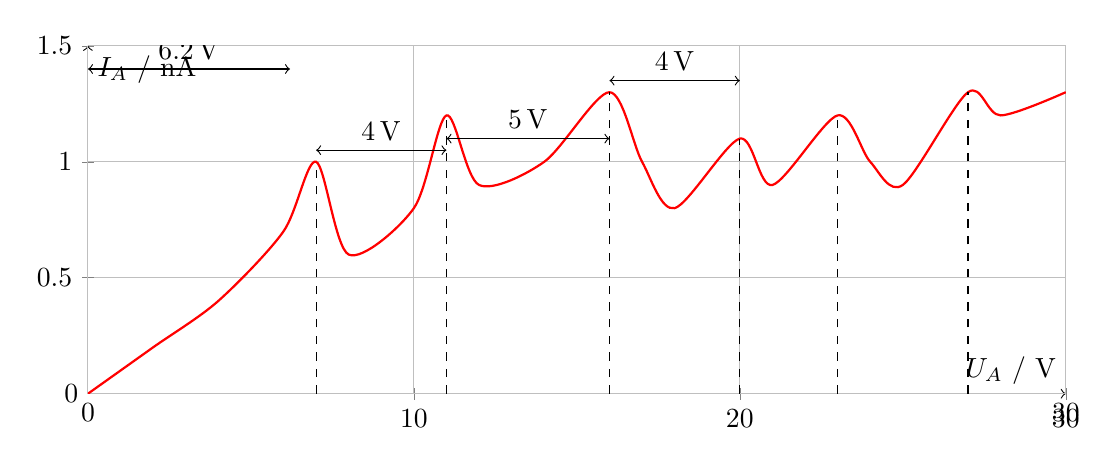
\begin{tikzpicture}
  \begin{axis}[
    width=14cm,
    height=6cm,
    xlabel={$U_A$ / V},
    ylabel={$I_A$ / nA},
    xmin=0, xmax=30,
    ymin=0, ymax=1.5,
    grid=major,
    axis lines=middle,
    axis line style={->},
    xtick={0,10,20,30},
    ytick={0,0.5,1.0,1.5},
    extra x ticks={0,30}, % Damit Pfeilspitzen am Ende sind
    extra x tick style={tick style={draw=none}, major tick length=0pt},
    extra y ticks={0},    % Damit Pfeil auf y-Achse
    extra y tick style={tick style={draw=none}, major tick length=0pt},
  ]

  % Fiktive Daten mit mehreren Peaks ähnlich einer Frank-Hertz-Kurve
  % U in V, I in nA
  \addplot[red,thick,smooth] coordinates {
    (0,0)
    (2,0.2)
    (4,0.4)
    (6,0.7)
    (7,1.0)   % Erster Peak
    (8,0.6)
    (10,0.8)
    (11,1.2)  % Zweiter Peak
    (12,0.9)
    (14,1.0)
    (16,1.3)  % Dritter Peak
    (17,1.0)
    (18,0.8)
    (20,1.1)  % Vierter Peak
    (21,0.9)
    (23,1.2)  % Fünfter Peak
    (24,1.0)
    (25,0.9)
    (27,1.3)  % Sechster Peak
    (28,1.2)
    (30,1.3)
  };

  % Vertikale gestrichelte Linien an den Peaks
  % Beispielhafte Positionen: 7 V, 11 V, 16 V, 20 V, 23 V, 27 V
  \addplot[dashed] coordinates {(7,0) (7,1.0)};
  \addplot[dashed] coordinates {(11,0) (11,1.2)};
  \addplot[dashed] coordinates {(16,0) (16,1.3)};
  \addplot[dashed] coordinates {(20,0) (20,1.1)};
  \addplot[dashed] coordinates {(23,0) (23,1.2)};
  \addplot[dashed] coordinates {(27,0) (27,1.3)};

  % Pfeile und Beschriftungen für Spannungsdifferenzen
  % Beispiel: Zwischen 7 V und 11 V ~4 V, zwischen 11 V und 16 V ~5 V usw.
  % Du kannst hier die tatsächlichen Werte und Positionen anpassen.

  % Pfeil von 7 V nach 11 V
  \draw[<->] (axis cs:7,1.05) -- (axis cs:11,1.05)
    node[midway,above] {$4\,\mathrm{V}$};

  % Pfeil von 11 V nach 16 V
  \draw[<->] (axis cs:11,1.1) -- (axis cs:16,1.1)
    node[midway,above] {$5\,\mathrm{V}$};

  % Pfeil von 16 V nach 20 V
  \draw[<->] (axis cs:16,1.35) -- (axis cs:20,1.35)
    node[midway,above] {$4\,\mathrm{V}$};

  % usw. je nach Wunsch weitere Pfeile ergänzen

  % Horizontaler Pfeil für eine Anfangsspannung z.B. 6.2 V
  \draw[<->] (axis cs:0,1.4) -- (axis cs:6.2,1.4)
    node[midway,above] {$6.2\,\mathrm{V}$};

  % y-Achsen-Beschriftung kannst du auch als node setzen, falls gewünscht.

  \end{axis}
\end{tikzpicture}
\end{document}




